\chapter{Geometrie auf der Kugeloberfläche\label{chapter:kugel}}
\lhead{Geometrie auf der Kugeloberfläche}
\begin{refsection}
\chapterauthor{Melina Staub und Fabian Schmid}

\section{Einleitung}

Seit jeher fasziniert den Menschen die Fahrt zur See. Nicht grundlos ist die Seefahrt eine der wichtigsten und ältesten Tätigkeiten der Menschheit. Der innerliche Drang neue Weltmeere und unbekannte Gebiete zu entdecken, die Fahrt zur See zu erleichtern und erträglicher zu machen, trieben die Menschen an, die Schiffe dieser Welt immer weiter zu entwickeln.

Die Idee der Kugelform der Erde ist älter als man zu denken vermag. Bereits der Schüler des antiken griechischen Philosophen Platon - Aristoteles schrieb in seiner Schrift \textit{Über den Himmel} aus dem 4. Jahrhundert v. Chr. etliche Gründe welche für die Gestallt der Erde als Kugel sprechen:\\

\begin{compactitem}
      \item Sämtliche schweren Körper streben zum Mittelpunkt des Alls. Da sie dies von allen Seiten her gleichmäßig tun und die Erde im Mittelpunkt des Alls steht, muss sie eine kugelrunde Gestalt annehmen. 
\item Bei von der Küste wegfahrende Schiffen wird der Rumpf vor den Segeln der Sicht verborgen. 
\item In südlichen Ländern erscheinen südliche Sternbilder höher über dem Horizont.
\item Der Erdschatten bei einer Mondfinsternis ist stets rund.
\end{compactitem}


Jedoch war um 1492 - der Zeit der Entdeckung Amerikas durch Christoph Kolumbus, die Idee der Erde in Kugelform noch sehr umstritten. Er erkannte anhand den Theorien und Erkenntnissen der alten Griechen, vor allem Aristoteles, das die Erde eine Kugel sein muss. \\
Doch mit seinem Vorschlag einen Seeweg über den Atlantik nach Indien zu finden und nicht wie üblich um Afrika zu segeln, stiess er beim beim portugiesischen König auf taube Ohren. Sein Plan Indien über eine Route nach Westen zu erreichen, widersprach dem gesunden Menschenverstand. Wäre die Erde wirklich eine Kugel und man befände sich auf der unteren Erdhalbkugel, würde man herunterfallen.\\
Doch auch der damals übliche Glaube an die Erde in Scheibenform brachte so einige Risiken mit sich. Was würde passieren, wenn die Flotte das Ende der Scheibe erreicht hatte? Würden sie über den Erdrand hinweggleiten und in den Abgrund stürzen?\\
Erst nach viel Überzeugungsarbeit durch Kolumbus, setzte er sich am Spanischen Hof durch und segelte über die Westliche Route über den Atlantik und entdeckte schlussendlich Amerika.

Der praktische und greifbare Beweis das die Erde eine Kugel ist, lieferte rund 30 Jahre später der Portugiese Fernando Magellan. Mit seiner Weltumsegelung und seiner Ankunft in den Philippinen, bewies er definitiv das die Erde eine Kugel ist.\\

Nun wollen wir uns die Frage stellen, wie die alten Seefahrer ohne GPS und jeglichen modernen Navigationssystemen auf hoher See wussten wo sie sich befinden und was haben die Sterne mit alldem zu tun? Reisen Sie mit uns zurück in eine Zeit mit Sextant, Kompass und Sternkarten. In die Zeit der Seefahrer und Entdecker.


\section{Geometrie auf der Ebene und der Kugel}

Euklid von Alexandria\footnote{%
Euklid war ein griechischer Mathematiker. Er lebte wahrscheinlich 3 Jahrhunderte vor Christus. In seinem berühmtesten Werk \textit{Euklids Elemente} fasst er die Arithmetik und Geometrie seiner Zeit zusammen. \textit{Euklids Elemente} war 2000 Jahre lang als Lehrbuch in gebrauch und war bis Mitte des 19. Jahrhunderts nach der Bibel das weit verbreitetste Buch der Weltliteratur.}  beschrieb die Grundbegriffe der ebenen Geometrie mittels Punkt, Geraden, Ebene, Winkel und Dreieck. Diese Dreiecke lassen sich mithilfe der ebenen Trigonometrie beschreiben. Dabei gelten die uns bekannten trigonometrischen Winkelfunktionen:\\

\text{Sinussatz:}
\begin{align*}
\frac{ a }{ sin(\alpha) } &= \frac{ b }{sin(\beta)} = \frac{ c }{ sin(\gamma) } = \frac{abc}{2A} = 2r\\
\end{align*}

\text{Cosinussatz:}
\begin{align*}
c^{ 2 } &= a^{ 2 } + b^{ 2 } - 2ab\cdot cos(\gamma)\\
b^{ 2 } &= a^{ 2 } + c^{ 2 } - 2ab\cdot cos(\beta)\\
a^{ 2 } &= b^{ 2 } + c^{ 2 } - 2ab\cdot cos(\alpha)
\end{align*}

Um Dreiecke auf der Kugeloberfläche zu berechnen, benötigt man die sphärische Trigonometrie. Die oben beschriebenen Sätze lassen sich auf der Kugel nicht anwenden, sie werden aber als Grundlage zur Herleitung der Sätze für das Kugeldreieck benötigt.

Die nachfolgenden Seiten thematisieren die Geometrie auf der Kugeloberfläche und wie sie in der Navigation eingesetzt werden kann.


\section{Gross- und Kleinkreise}

Eine Kugeloberfläche lässt sich in zwei verschiedene Kreisarten einteilen -  Gross- und Kleinkreise. 
Wir betrachten als erstes die Grosskreise:

\begin{definition}
Ein Grosskreis ist ein größtmöglicher Kreis auf einer Kugeloberfläche. Sein Mittelpunkt fällt immer mit dem Mittelpunkt der Kugel zusammen und ein Schnitt auf dem Grosskreis teilt die Kugel in jedem Fall in zwei („gleich große“) Hälften.
\end{definition}

Es gibt unendlich viele Möglichkeiten, eine Kugel in zwei gleich grosse Stücke zu zerschneiden, 
daher gibt es auch unendlich viele Grosskreise. Wenn wir die Grosskreise auf einer Kugel mit diesen auf der Erde beschreiben, sprechen wir von den Längengraden aber auch der Äquator beschreibt einen Grosskreis.
Ein Elementarer Bestandteil bilden die Grosskreise in der sphärischen Trigonometrie. Mithilfe der Schnittpunkte verschiedener Grosskreise, lässt sich ein Sphärisches Dreieck bilden auf welchem sich die sphärische Trigonometrie anwenden lässt.

\begin{center}
        \includegraphics[width=0.3\textwidth]{kugel/Beispielbild.jpg}
    \captionof{figure}{BILD GROSSKREISE}
\end{center}

\begin{definition}
Unter Kleinkreis versteht man jene Kreise auf einer Kugeloberfläche, deren Ebenen nicht den Kugelmittelpunkt enthalten.
\end{definition}

Die Kleinkreise eignen sich im Gegensatz zu den Grosskreisen \textit{nicht} für die sphärische Trigonometrie. 
Sie werden lediglich zur Bestimmung der Messgrössen, Winkelabstände oder des Höhenwinkels eines Gestirns verwendet. 

Wenn wir die Kleinkreise auf die Erdoberfläche projizieren betrachten wir die Breitengrade.

\begin{center}
        \includegraphics[width=0.3\textwidth]{kugel/Beispielbild.jpg}
    \captionof{figure}{BILD KleinKREISE}
\end{center}


\section{Sphärische Dreiecke / Kugeldreieck}

\begin{center}
        \includegraphics[width=0.9\textwidth]{kugel/Dreieckarten.jpg}
    \captionof{figure}{Dreiecksarten auf der Kugeloberfläche}
\end{center}

Der Begriff Sphärisches Dreieck oder Kugeldreieck ist ein sehr weitläufiger Begriff. 
Dabei können wir den Begriff in drei für uns wesentliche Dreiecke unterteilen:\\

\begin{compactitem}
\item Kugelzweieck
\item Nicht Eulersche’Dreiecke
\item Eulersche’Dreiecke
\end{compactitem}

\subsection{Kugelzweieck}

Zwei Grosskreise auf der Kugeloberfläche zerlegen diese in vier gleich grosse Kugelzweiecke. 
Jedes dieser Dreieckseiten hat die Länge
$180^{\circ}$ oder $\pi$
Der Flächeninhalt wird dabei nur durch den Winkel $\alpha$ zwischen den beiden Grosskreisen bestimmt.

\begin{center}
        \includegraphics[width=0.3\textwidth]{kugel/Zweieck.jpg}
    \captionof{figure}{Bildung von Zweiecken durch Grosskreise}
\end{center}

Um den Flächeninhalt des Zweiecks zu erhalten, benötigen wir den Flächeninhalt der Kugel

\begin{align*}
A_{ Kugel } &= 4 \pi r^{2}
\end{align*}

Diesen müssen wir noch mit dem Kugelsegment des Winkels $\alpha$ multiplizieren um dem Flächeninhalt des Zweiecks zu erhalten

\begin{equation}
A_{ Zweieck } = 4 \pi r^{2} \cdot \frac{ \alpha }{ 2 \pi }
\end{equation}

HIER NOCH EIN SATZ

\subsection{Nicht Eulersche’ Dreiecke}

BLABLA

\subsection{Eulersche’ Dreiecke}

Legt man drei Grosskreise auf eine Kugeloberfläche, bilden sich dabei acht Dreiecke. 
Ein solches Dreieck heisst Eulersches’Dreieck\footnote{%
Leonard Euler (1707-1783), berühmter Schweizer Mathematiker und Physiker. 
Nicht Eulersche’Dreiecke erhält man, indem man das Äussere des Dreieckes ABC betrachtet.} 
Diese Dreiecke werden weder durch die Verlängerung ihrer Seiten durchschnitten, 
noch haben sie Dreiecksseiten welche grösser als $180^{\circ}$ sind.

\begin{center}
        \includegraphics[width=0.4\textwidth]{kugel/Zweiecke.jpg}
    \captionof{figure}{Drei Grosskreise bilden ein sphärisches Dreieck}
\end{center}

In den nachstehenden Erklärungen und Herleitungen, sprechen wir ausschliesslich von Eulerschen’Dreiecken, da die umgeformten Winkelsätze der ebenen Trigonometrie nur auf diese Art von Kugeldreiecken angewendet werden kann.

$A_{ \overline{ ABC }}$ ist die Fläche des Dreieckes auf der Kugeloberfläche
In der ebenen Trigonometrie liegt die Winkelsumme eines Dreiecks bei
$180^{\circ}$.

Anders aber in der sphärischen Trigonometrie. Obschon sie einige Gemeinsamkeiten zur ebenen Trigonometrie aufweist, kann man nicht alles übernehmen.
So auch nicht wie Winkelsumme in einem sphärischen Dreieck.
Diese liegt bei:

\[
\begin{aligned}
\pi
&-
3\pi
&
&\text{\bigg \vert}
&
180^{\circ}
&-
540^{\circ}
\end{aligned}
\]

daraus lässt sich ableiten, das ein einzelner Winkel nicht grösser als $\pi$ oder $180^{\circ}$ sein darf. Ansonsten ist es kein Eulersches’Dreieck und wir dürfen die sphärische Trigonometrie nicht anwenden.\\
Wichtig anzumerken ist, dass die Seiten immer in Radiant beschrieben werden und nicht im Längenmass Meter wie wir es uns gewohnt sind. 
Bei den Dreiecksseiten handelt es sich um Kreisbögen und keine Strecken.

\section{Dreiecksfläche}

\begin{center}
        \includegraphics[width=0.3\textwidth]{kugel/Beispielbild.jpg}
    \captionof{figure}{BILD FLäche dreieck}
\end{center}

\begin{align*}
\text{Zweieck A}
&=
\overline{ABC} + \overline{A'BC} = 2 \alpha r^{ 2 } = A_{ \alpha }\\
\text{Zweieck B}
&=
\overline{ABC} + \overline{AB'C} = 2 \beta r^{ 2 } = A_{ \beta }\\
\text{Zweieck C}
&=
\overline{ABC} + \overline{ABC'} = 2 \gamma r^{ 2 } = A_{ \gamma }
\end{align*}

\begin{align*}
A_{ \alpha } + A_{ \beta } + A_{ \gamma } &= \frac{ 4\pi r^{ 2 } }{ 2 } + 2A_{ \overline{ ABC }} \\
2\alpha r^{ 2 } + 2\beta r^{ 2 } + 2\gamma r^{ 2 } &= \frac{ 4\pi r^{ 2 } }{ 2 } + 2A_{ \overline{ ABC }} \parallel:2\\
\alpha r^{ 2 } + \beta r^{ 2 } + \gamma r^{ 2 } &= \pi r^{ 2 } + A_{ \overline{ ABC }} \parallel-\pi r^{ 2 }\\
r^{ 2 }\left(\alpha + \beta + \gamma - \pi\right) &= A_{ \overline{ ABC }}
\end{align*}


\section{Sphärischer Exzess}
Die Winkelsumme sphärischer Dreiecke ist immer \textgreater \,  $\pi$.

\begin{align*}
\pi < \alpha + \beta + \gamma
\end{align*}

Der sphärische Exzess gibt dabei an, wie stark die Winkelsumme von $\pi$ abweicht.

\begin{align*}
\pi + \epsilon &= \alpha + \beta + \gamma \\
\end{align*}

Lösen wir nach $\epsilon$ auf:

\begin{equation}
\epsilon = \alpha + \beta + \gamma - \pi
\end{equation}

\begin{center}
        \includegraphics[width=0.3\textwidth]{kugel/Beispielbild.jpg}
    \captionof{figure}{BILD SPHÄRISCHER EXZESS}
\end{center}

Würde der sphärische Exzess in der ebenen Trigonometrie angewendet, wäre dieser = 0. 
Bezieht man das auf die Erde und somit einer Kugel, kann man mit Hilfe eines beliebigen sphärischen Dreieckes und dessen Flächeninhalt auf den Radius der Kugel schliessen.

\subsection{Grenzfall - Satz von Legendre}

\begin{quote} \textit{Ein kleines sphärisches Dreieck kann näherungsweise 
wie ein ebenes Dreieck mit denselben Seiten berechnet 
werden, wenn alle Winkel des ebenen Dreiecks die um 
je ein Drittel des sphärischen Exzesses verminderten 
Winkel des sphärischen Dreiecks nimmt.} \end{quote}
\begin{flushright} - Adrien-Marie Legendre (1752-1833), Paris 1787
\end{flushright}

Diese Aussage zeigt den Zusammenhang zwischen der 
Trigonometrie in der Ebene sowie in auf der Kugel
auf. Im speziellen bei sehr kleinen sphärischen 
Dreiecken ist die Winkelsumme nur unwesentlich 
grösser als $180^{\circ}$. Des Weiteren kann gesagt werden,
dass der sphärische Exzess gleichmässig auf alle
Winkel aufgeteilt wird.
Wichtig anzumerken ist, dass der Satz von Legendre 
für grosse, aber endliche Radien $r$ gilt.

\begin{center}
        \includegraphics[width=0.3\textwidth]{kugel/Beispielbild.jpg}
    \captionof{figure}{BILD SKIZZE GROSSER RADIUS/KLEINE KRÜMMUNG, KLEINER RADIUS/GROSSE KRÜMMUNG}
\end{center}


\section{Sphärisch Analoge Winkelfunktionen}

\subsection{Sphärischer Sinussatz}

\begin{center}
        \includegraphics[width=0.3\textwidth]{kugel/Beispielbild.jpg}
    \captionof{figure}{BILD SINUSSATZ}
\end{center}


Wir betrachten das folgende sphärische Dreieck auf einem Teilstück der Kugeloberfläche mit dem Radius $R= \overline{MA} = \overline{MB} = \overline{MC}$. Danach fügen wir ein ebenes Dreieck $\triangle=\overline{ADE}$ in das Kugelstück ein, welches den Eckpunkt $A$ des sphärischen Dreiecks beinhaltet und eine Abbildung des sphärischen Dreieckes bildet.

Es gilt

\begin{align*}
\overline{AD} &= R \cdot sin (c) \\
hA = \overline{AF} &= \overline{AD} \cdot sin(\beta) = R \cdot sin(c) \cdot sin(\beta)  
\end{align*}

Aus einer anderen Sichtweise kann man auch schreiben

\begin{align*}
h_{A} = R \cdot sin(b) \cdot sin(\gamma)  
\end{align*}

Durch gleichsetzen dieser Ausdrücke ergibt sich

\begin{align*}
R \cdot sin(c) \cdot sin(\beta) &= R \cdot sin(b) \cdot sin(\gamma) \\
\Rightarrow \quad \quad
sin(c) \cdot sin(\beta) &= sin(b) \cdot sin(\gamma) \\
\Rightarrow \quad \quad
\frac{sin (b)}{sin (c)} &= \frac{sin (\beta)}{sin (\gamma)}
\end{align*}

Analog dazu könnte man auch die Höhe $h_{B}$ nehmen und würde erhalten

\begin{align*}
sin(c) \cdot sin(\alpha) &= sin(a) \cdot sin(\gamma) \\
\Rightarrow \quad \quad
\frac{sin (a)}{sin (c)} &= \frac{sin (\alpha)}{sin (\gamma)}
\end{align*}

Aus diesen Erkenntnissen lässt sich der Sinussatz zusammenfassen

\begin{satz}[\textit{Der sphärische Sinussatz verhaltet sich wie der Sinus der Seiten wie der Sinus der Gegenwinkel, dies lässt sich beschreiben}]
\label{skript:kugel:satz:Sinussatz}
\index{Sinussatz}
\end{satz}

\begin{align*}
\sin(a) : \sin(b) : \sin(c) &= \sin(\alpha) : \sin(\beta) : \sin(\gamma) \\
 \\
\frac{sin(\alpha)}{sin(a)} &= \frac{sin(\beta)}{sin(b)} = \frac{sin(\gamma)}{sin(c)}
\end{align*} 


\subsection{Seitenkosinussatz}

Es sei das Stück einer Kugel mit dem sphärischen Dreieck $ABC$ und den Winkeln $\alpha, \beta, \gamma$ und den Seiten $a, b, c$. Die Senkrechten durch den Mittelpunkt, schneiden dabei die Eckpunkte des sphärischen Dreieckes. Wir erstellen in der Ebene ein Ähnliches Dreieck $A’B’C’$.

\begin{center}
        \includegraphics[width=0.3\textwidth]{kugel/Beispielbild.jpg}
    \captionof{figure}{BILD SEITENKOSINUS}
\end{center}

Dabei lassen sich die Strecken nach den uns bekannten Regeln der Trigonometrie beschreiben:

\begin{align*}
\overline{C'A'} &= d\cdot {tan(b)} \\
\overline{C'B'} &= d\cdot {tan(a)} \\
\overline{MA'} &= \frac{ d }{cos(b)} \\
\overline{MB'} &= \frac{ d }{cos(a)}
\end{align*} 

Dabei schreibt sich der Kosinussatz der Ebene wie folgt

\begin{align*}
c^{ 2 } &= a^{ 2 } + b^{ 2 } - 2ab \cdot cos(\gamma)
\end{align*}

Daher gilt für das Dreieck $A’,B’,C’$

\begin{align*}
\triangle \overline{A'B'}^{ 2 } &= \overline{ C'B' }^{ 2 } + \overline{ C'A' }^{ 2 } - 2 \cdot \overline{C'B'} \cdot \overline{ C'A' } \cdot cos(\gamma) \\
\Rightarrow \quad \quad
\triangle \overline{A'B'}^{ 2 } &= d^{ 2 } \cdot \left(\left(tan^{ 2 }(a) + tan^{ 2 }(b)\right) - 2\cdot tan(a) \cdot tan(b) \cdot cos(\gamma)\right)
\end{align*}


das gilt ebenso für das Dreieck $MA’B’$

\begin{align*}
\triangle \overline{ MA'B' }^{ 2 } &= \overline{ MB' }^{ 2 } + \overline{ MA' }^{ 2 } - 2\cdot \overline{ MB'} \cdot \overline{ MA' } \cdot cos(c) \\
\Rightarrow \quad \quad
\overline{ A'B'}^{ 2 } &= \left(\frac{ d }{ cos(a) }  \right)^{ 2 } + \left(\frac{ d }{ cos(b)}  \right)^{ 2 } - 2 \cdot \frac{ d }{ cos(a)} \cdot \frac{ d }{ cos(b)} \cdot cos(c)
\end{align*}


Im Einheitskreis betrachtet ergibt dies

\begin{align*}
\overline{ A'B' }^{ 2 } &= d^{ 2 } \cdot \left(\left(\frac{ 1 }{ cos(a) }  \right)^{ 2 } + \left(\frac{ 1 }{ cos(b) }  \right)^{ 2 } - 2 \cdot \frac{ 1 }{ cos(a)} \cdot \frac{ 1 }{ cos(b)} \cdot cos(c)\right)
\end{align*}


Durch berücksichtigen von $\frac{1}{\cos^{2}(x)}=\tan^{2}(x)+1$ folgt

\begin{align*}
\overline{ A'B'}^{ 2 } &= d^{ 2 } \cdot \left(\left(tan^{ 2 }(a) + tan^{ 2 }(b)\right) - 2 \cdot tan(a) \cdot tan(b) \cdot cos(\gamma)\right) \\
\Rightarrow \quad \quad
\overline{ A'B'}^{ 2 } &= d^{ 2 } \cdot \left(\left(tan^{ 2 }(a) + 1\right) + \left(tan^{ 2 }(b) + 1\right) - \left(2 \cdot \frac{cos(c)}{cos(a) \cdot cos(b)}\right)\right)
\end{align*}


Durch gleichsetzen dieser beiden Ausdrücke folgt

\begin{align*}
2 \cdot tan(a) \cdot tan(b) \cdot cos(\gamma) &= 2 \cdot \frac{cos(c)}{cos(a) \cdot cos(b)}
\end{align*}


% IRGENDWIE KOMME ICH DA NICHT WEITER…. es fehlt noch mal ½ und dan mit cos a und cos b multiplizieren

Durch zyklische Vertauschung der Variablen erhält man den 
\begin{satz}[Seitenkosinussatz]
\label{skript:kugel:satz:seitenkosinussatz}
\index{Seitenkosinussatz}
\end{satz}

\begin{align*}
{cos(a)} &= {cos(b)} \cdot {cos(c)} + {sin(b)} \cdot {sin(c)} \cdot {cos(\alpha)}\\
{cos(b)} &= {cos(c)} \cdot {cos(a)} + {sin (c)} \cdot {sin(a)} \cdot {cos(\beta)}\\
{cos(c)} &= {cos(a)} \cdot {cos(b)} + {sin(a)} \cdot {sin(b)} \cdot {cos(\gamma)}\\
\end{align*}




\subsection{Winkelkosinussatz}

\begin{center}
        \includegraphics[width=0.3\textwidth]{kugel/Beispielbild.jpg}
    \captionof{figure}{BILD WINKELKOSINUS / POLARDREIECK}
\end{center}





\section{Navigation auf See}
Das besondere an Seekarten ist die Inhaltliche Ausrichtung. Anders wie Landkarten muss sie Informationen enthalten welche für den Kapitän und seine Besatzung von grosser Bedeutung sind. Vor allem in Küstennähe ist das navigieren eines Schiffes besonders gefährlich. So enthalten Seekarten etwas über Wassertiefen, Bodenbeschaffenheiten, Gezeiten, Küstenlinien, Landzungen und Windrichtungen.
Der Hauptunterschied dabei ist, das auf der Landkarte feste Positionen definiert und aufgezeigt werden, das einzige was sich verändert ist der Reisende selbst. Bei der Seekarte ist das anders, es werden veränderliche Einwirkungen der Natur festgehalten.

Dieser kleine Unterschied zeigt die Notwendigkeit auf, die Position und den Kurs seines Schiffes auf See immer ermitteln zu können.


\section{Geographische Koordinaten}

Nachdem klar war, das die Erde eine Kugel ist, wurde diese in ein Gradnetz aufgeteilt. Dabei wurden die Angaben für eine exakte Ortsbestimmung klar definiert und die bis heute gültigen Koordinaten bestimmt.
Dabei muss man sich nochmals in Erinnerung rufen, dass sich die Erde in 24h einmal um ihre eigene Achse dreht. Nach $360 ^{\circ}$ 
und somit einer vollen Umdrehung, steht sie wieder in ihrer Ursprungsposition und ein neuer Tag beginnt.

Die Koordinaten setzen sich aus folgenden Komponenten zusammen:

\[
\begin{aligned}
&\text{Grad } (^{\circ})
&
&\text{\bigg \vert}
&
&\text{Bogenminuten } (`)
&
&\text{\bigg \vert}
&
&\text{Bogensekunden } (``)
\end{aligned}
\]

Die Erdoberfläche wurde in je 360 Breiten- und Längengrade eingeteilt. Die Breitengrade haben zueinander einen Abstand von 111.31 km, dies entspricht auch dem Abstand der Längengrade am Äquator mit Zunehmender Nähe zu den Polen, nimmt dieser Abstand ab.

\[
\begin{aligned}
&1^{\circ}
&
&\text{\bigg \vert}
&
&4 \text{ Minuten}
&
&\text{\bigg \vert}
&
&111.31\text{ km}
\end{aligned}
\]

Berechnet man nun die Erdumdrehung von 360°, erhält man genau den Erdumfang am Äquator: \begin{align*} 40’074 \text{ km.}\end{align*}

Dabei geben die Bogenminuten und -sekunden dem Standort die gewünschte Exaktheit. Mit den vollständigen Koordinaten lässt sich der Standort auf einer Landkarte exakt bestimmen und einzeichnen.

\subsection{Erdachsenneigung}

\begin{center}
        \includegraphics[width=0.3\textwidth]{kugel/Beispielbild.jpg}
    \captionof{figure}{BILD ERDNEIGUNG}
\end{center}

Lorem ipsum dolor sit amet. Lorem ipsum dolor sit amet, consetetur sadipscing elitr, sed diam nonumy eirmod tempor invidunt ut labore et dolore magna aliquyam erat, sed diam voluptua. At vero eos et accusam et justo duo dolores et ea rebum. Stet clita kasd gubergren, no sea takimata sanctus est Lorem ipsum dolor sit amet.

\subsection{Zeitzonen der Erde}
Wenn man nun die verschiedenen Zeitzonen der Erde betrachtet, macht die Verschiebung von jeweils einer Stunde durchaus Sinn, es lässt sich auf die Längengrade schliessen.
Zwischen den verschiedenen Zeitzonen liegen 15 Längengrade:
\begin{align*}
\text{15 Längengrade à 4 Minuten = 60 Minuten Zeitverschiebung = ca. 1665 km}
\end{align*}

Dabei ist die Zeitzone in welcher Mitte sich der Greenwich Meredian befindet die \textit{Greenwich Mean Time (GMT)} welche bis 1928 als Weltzeit galt. Im Jahr 1972 wurde diese umbenannt in die \textit{Coordinated Universal Time (UTC)} und wir von da an als Weltzeit $\pm$ 0.00 verwendet.


\section{Der Breitengrad}
Die Breitengrade bilden die bereits genannten Kleinkreise auf der Kugeloberfläche. Sie verlaufen in einem Abstand von genau 111 km parallel zum Äquator. Dabei stellt  dieser genau die Mitte zwischen Nord- und Südpol dar und teilt die Erdkugel in zwei gleiche Hälften. Somit wird von nördlicher und südlicher Breite gesprochen, je nach dem auf welcher Halbkugel man sich befindet.

\begin{center}
        \includegraphics[width=0.3\textwidth]{kugel/Beispielbild.jpg}
    \captionof{figure}{BILD SKIZZE DER GEOGRAFISCHEN BREITE ERDKUGEL}
\end{center}


\subsection{Geografische Breite $\phi$}
\begin{definition}
Die geografische Breite eines Standortes ist nichts anderes, als der Winkel am Erdmittelpunkt zwischen der Ebene des Äquators und der Geraden zum Standpunkt auf der Erdoberfläche.
\end{definition}

\begin{center}
        \includegraphics[width=0.3\textwidth]{kugel/Beispielbild.jpg}
    \captionof{figure}{BILD SKIZZE DER GEOGRAFISCHEN BREITE MIT WINKEL}
\end{center}


\subsection{Navigation mit den Breitengraden}
Da der Breitengrad bereits sehr früh ziemlich präzise bestimmt werden könnte, nutzten bereits die Seefahrer um Christoph Kolumbus den Breitengrad zur Navigation ihrer Flotten.
Den dieser lässt sich ziemlich einfach aus dem höchsten Sonnenstand oder einem Fixstern bestimmen. Dabei wird mit einem Jakobsstab\footnote{%
Der Jakobsstab ist ein früheres astronomisches Instrument zur Winkelmessung und wurde vor allem in der Seefahrt verwendet. Er ist in der Nautik der Vorläufer des Sextanten.} (später Sextant\footnote{%
Der Sextant ist ein nautisches Messinstrument zur Winkelmessung von Horizont und Fixstern (Gestirn)}) der Winkel zwischen dem Horizont und dem Fixstern gemessen. Der Winkel welchen man erhält, zieht man von 90° ab und erhält somit die geografische Breite. \\

\begin{center}
        \includegraphics[width=0.3\textwidth]{kugel/Beispielbild.jpg}
    \captionof{figure}{BILD SKIZZE ERMITTLUNG DES BREITENGRADES}
\end{center}

Wenn man sich auf der Nordhalbkugel befindet, ist der Polarstern ein sehr guter Fixstern. Befindet sich ein Schiff nun sehr nahe am Nordpol, steht dieser nahezu senkrecht am Himmelszelt bei $90^{\circ}$. Würde es aber nahe dem Äquator stehen, erscheint dieser am Horizont bei $0^{\circ}$.

\subsection{Korrekturbeiwert}
Lorem ipsum dolor sit amet. Lorem ipsum dolor sit amet, consetetur sadipscing elitr, sed diam nonumy eirmod tempor invidunt ut labore et dolore magna aliquyam erat, sed diam voluptua. At vero eos et accusam et justo duo dolores et ea rebum. Stet clita kasd gubergren, no sea takimata sanctus est Lorem ipsum dolor sit amet.


\section{Der Längengrad}
Die Längengrade bilden die bereits genannten Grosskreise auf der Kugeloberfläche.
Sie schneiden den Äquator im rechten Winkel, haben dort einen Abstand von 111 km zueinander und verbinden die Pole. Anders wie bei der geografischen Breite, ist in der Natur kein Längengrad gegeben welcher den Nullpunkt darstellt.

\begin{center}
        \includegraphics[width=0.3\textwidth]{kugel/Beispielbild.jpg}
    \captionof{figure}{BILD SKIZZE DER GEOGRAFISCHEN LÄNGE ERDKUGEL}
\end{center}


\subsection{Geografische Länge $\lambda$}
\begin{definition}
Die geografische Länge ist der Winkel an der Erdachse zum Nullmeridian.
\end{definition}

\subsection{Navigation mit den Längengraden}
Die geografische Länge lässt sich nicht so einfach bestimmen wie deren Breite. Für die Berechnung auf See benötigt man eine Referenzzeit eines Ortes mit bekannter Länge.
In der Zeit der Entdecker gab es noch keine mechanischen Uhren. Die Sonnenuhr war zudem ungeeignet, da diese nur die Uhrzeit am Standort mass und nicht die am Referenzort selbst. Die erste Pendeluhr wurde erst Mitte des 17. Jahrhunderts erfunden, was in der Schifffahrt aber auch nicht die Lösung brachte.\\
Pendeluhren auf einem Schiff sind ungeeignet, da das Pendel mit dem Wellengang aus dem Takt gebracht wird und somit die Uhr falsch geht.
Zu ungenau und gegen äussere Erschütterungen zu empfindlich waren später auch die federgetriebenen Uhren und die Unruh. Dazukamen die verschiedenen Klimazonen welche ein Schiff zu durchqueren hatten. Das Metall zog sich viel zu fest zusammen oder dehnte sich aus, was dazu führte das die Uhr unregelmässig lief.

Das sogenannte „Längenproblem“ stellte nicht nur bei der Navigation auf See ein Problem dar, es ergaben sich auch wirtschaftliche Konsequenzen. Die Schiffe mussten bis zur gewünschten geografischen Breite navigieren und segelten dann den Breitengrad entlang. Dabei waren die Schiffe oft Wochenlang unterwegs und segelten die „Breiten ab“ um an die gewünschte Position zu kommen. Dies führte zu erheblichen Zeitverlusten und viel längeren Reisezeiten.


\section{The Board of Longitude - Das Längenproblem}
Das Längenproblem beschäftigte alle grossen Seefahrernationen Europas. Wenn man bedenkt das sich Werte in einer  Höhe von halben britischen Staatshaushalten auf verloren gegangenen Schiffen befanden, erkennt man die Dringlichkeit für eine zuverlässige und genaue Navigation auf See.\\


\begin{compactitem}
\item £ 20’000 - Abweichung von max. einem halben Grad
\item £ 15’000 - Abweichung von zwei Drittel Grad
\item £ 10’000 - Abweichung von max. $1 ^{\circ}$
\end{compactitem}

\subsection{John Harrison}

\begin{center}
        \includegraphics[width=0.3\textwidth]{kugel/JohnHarrison.jpg}
    \captionof{figure}{BILD JOHN HARRISON}
\end{center}





\begin{center}
        \includegraphics[width=0.2\textwidth]{kugel/HarrisonH4.jpg}
    \captionof{figure}{BILD Harrison's H4}
\end{center}


\subsection{Tobias Mayer}

\begin{center}
        \includegraphics[width=0.3\textwidth]{kugel/TobiasMayer.jpg}
    \captionof{figure}{BILD TOBIAS MAYER}
\end{center}



\begin{center}
        \includegraphics[width=0.3\textwidth]{kugel/Mondkarte.jpg}
    \captionof{figure}{BILD Mondkarte}
\end{center}


Uhren mit einer Abweichung von einer Minute Abweichung pro Tag (





\section{Nautische Dreieck}

\begin{center}
        \includegraphics[width=0.3\textwidth]{kugel/Beispielbild.jpg}
    \captionof{figure}{BILD NAUTISCHES DREIECK}
\end{center}

$\Rightarrow$



\section{Die Vermessung der Welt}
Wir schreiben das Jahr 1818 und kehren in die Zeit des Mathematikers Carl Friedrich Gauss zurück. Neben dem liebevoll genannten „kleinen Gauss“ und anderen herausragenden Mathematischen Leistungen, beschäftigte er in den Folgejahren mit der Vermessung des Königreichs Hannovers und verfasste auf 61 Blättern das Kartenwerk \textit{Gauss’sche Landesaufnahme der 1815 durch Hannover erworbenen Gebiete}.
\cite{skript:tabea}


\begin{equation}
\dot s(t)=|\dot c(t)|
\quad
\text{ mit der Anfangsbedingung }\quad s(a)=0.
\label{skript:kruemmung:laengedgl}
\end{equation}


\cite{lin1973}


AUFGABE

Hubble Teleskop 
24. April 1990


\chapter{Lichtablenkung an einem Galaxiencluster\label{chapter:thema}}
\lhead{Lichtablenkung an einem Galaxiencluster}
\begin{refsection}
\chapterauthor{Pascal Stump}

\section{Einleitung}
\rhead{Einleitung}
Wenn ein sehr massereiches Objekt zwischen einem Betrachter und einer
Lichtquelle platziert ist, tritt ein Gravitationslinseneffekt auf.  In
der Abbildung \ref{fig:lrg3-757} sieht man ein Beispiel, bei welchem
die Vordergrund-Galaxie (gelb/orange) praktisch in einer Linie zur
Hintergrund-Galaxie (blau) steht.  Durch die beinahe optimale
Ausrichtung in einer Linie wird die Hintergrund-Galaxie zu einem
Kreis verzerrt.  Der dabei entstehende Kreis wird auch Einsteinring
genannt.

Wenn die Vordergrund-Galaxie nicht rotationssymmetrisch ist, kann die
Hintergrund-Galaxie zu einzelnen Punkten verzerrt werden, so zu sehen
in der Abbildung \ref{fig:einsteinkreuz}.  Dabei ist die
Vordergrund-Galaxie wieder in der Mitte zu finden und die vier
umliegenden Punkte sind die verzerrte Hintergrund-Galaxie.

Ein drittes Beispiel des Gravitationslinseneffekts ist in Abbildung
\ref{fig:abell} zu finden.  Dabei ist nicht nur eine Galaxie als Linse
zuständig, sondern ein Galaxiencluster.  Die Vordergrund-Galaxien ist
wiederum die gelb, orange farbigen Galaxien.  Man sieht schön, dass
die Hintergrund-Galaxien zu Streifen verzogen werden und nicht mehr zu
einem ganzen Kreis, da die Ausrichtungen zueinander nicht optimal
sind.

\begin{figure}
  \centering
  \includegraphics[width=\textwidth]{cluster/images/LRG_3-757}
  \caption{Einsteinring (LRG 3-757; ESA/Hubble \& NASA)
    \cite{nasa:einsteinring, wiki:einsteinring}}
  \label{fig:lrg3-757}
\end{figure}

\begin{figure}
  \centering
  \includegraphics[width=.7\textwidth]{cluster/images/Einstein_cross}
  \caption{Einsteinkreuz (G2237+0305; NASA, ESA \& STScl)
    \cite{wiki:einsteinkreuz}}
  \label{fig:einsteinkreuz}
\end{figure}

\begin{figure}
  \centering
  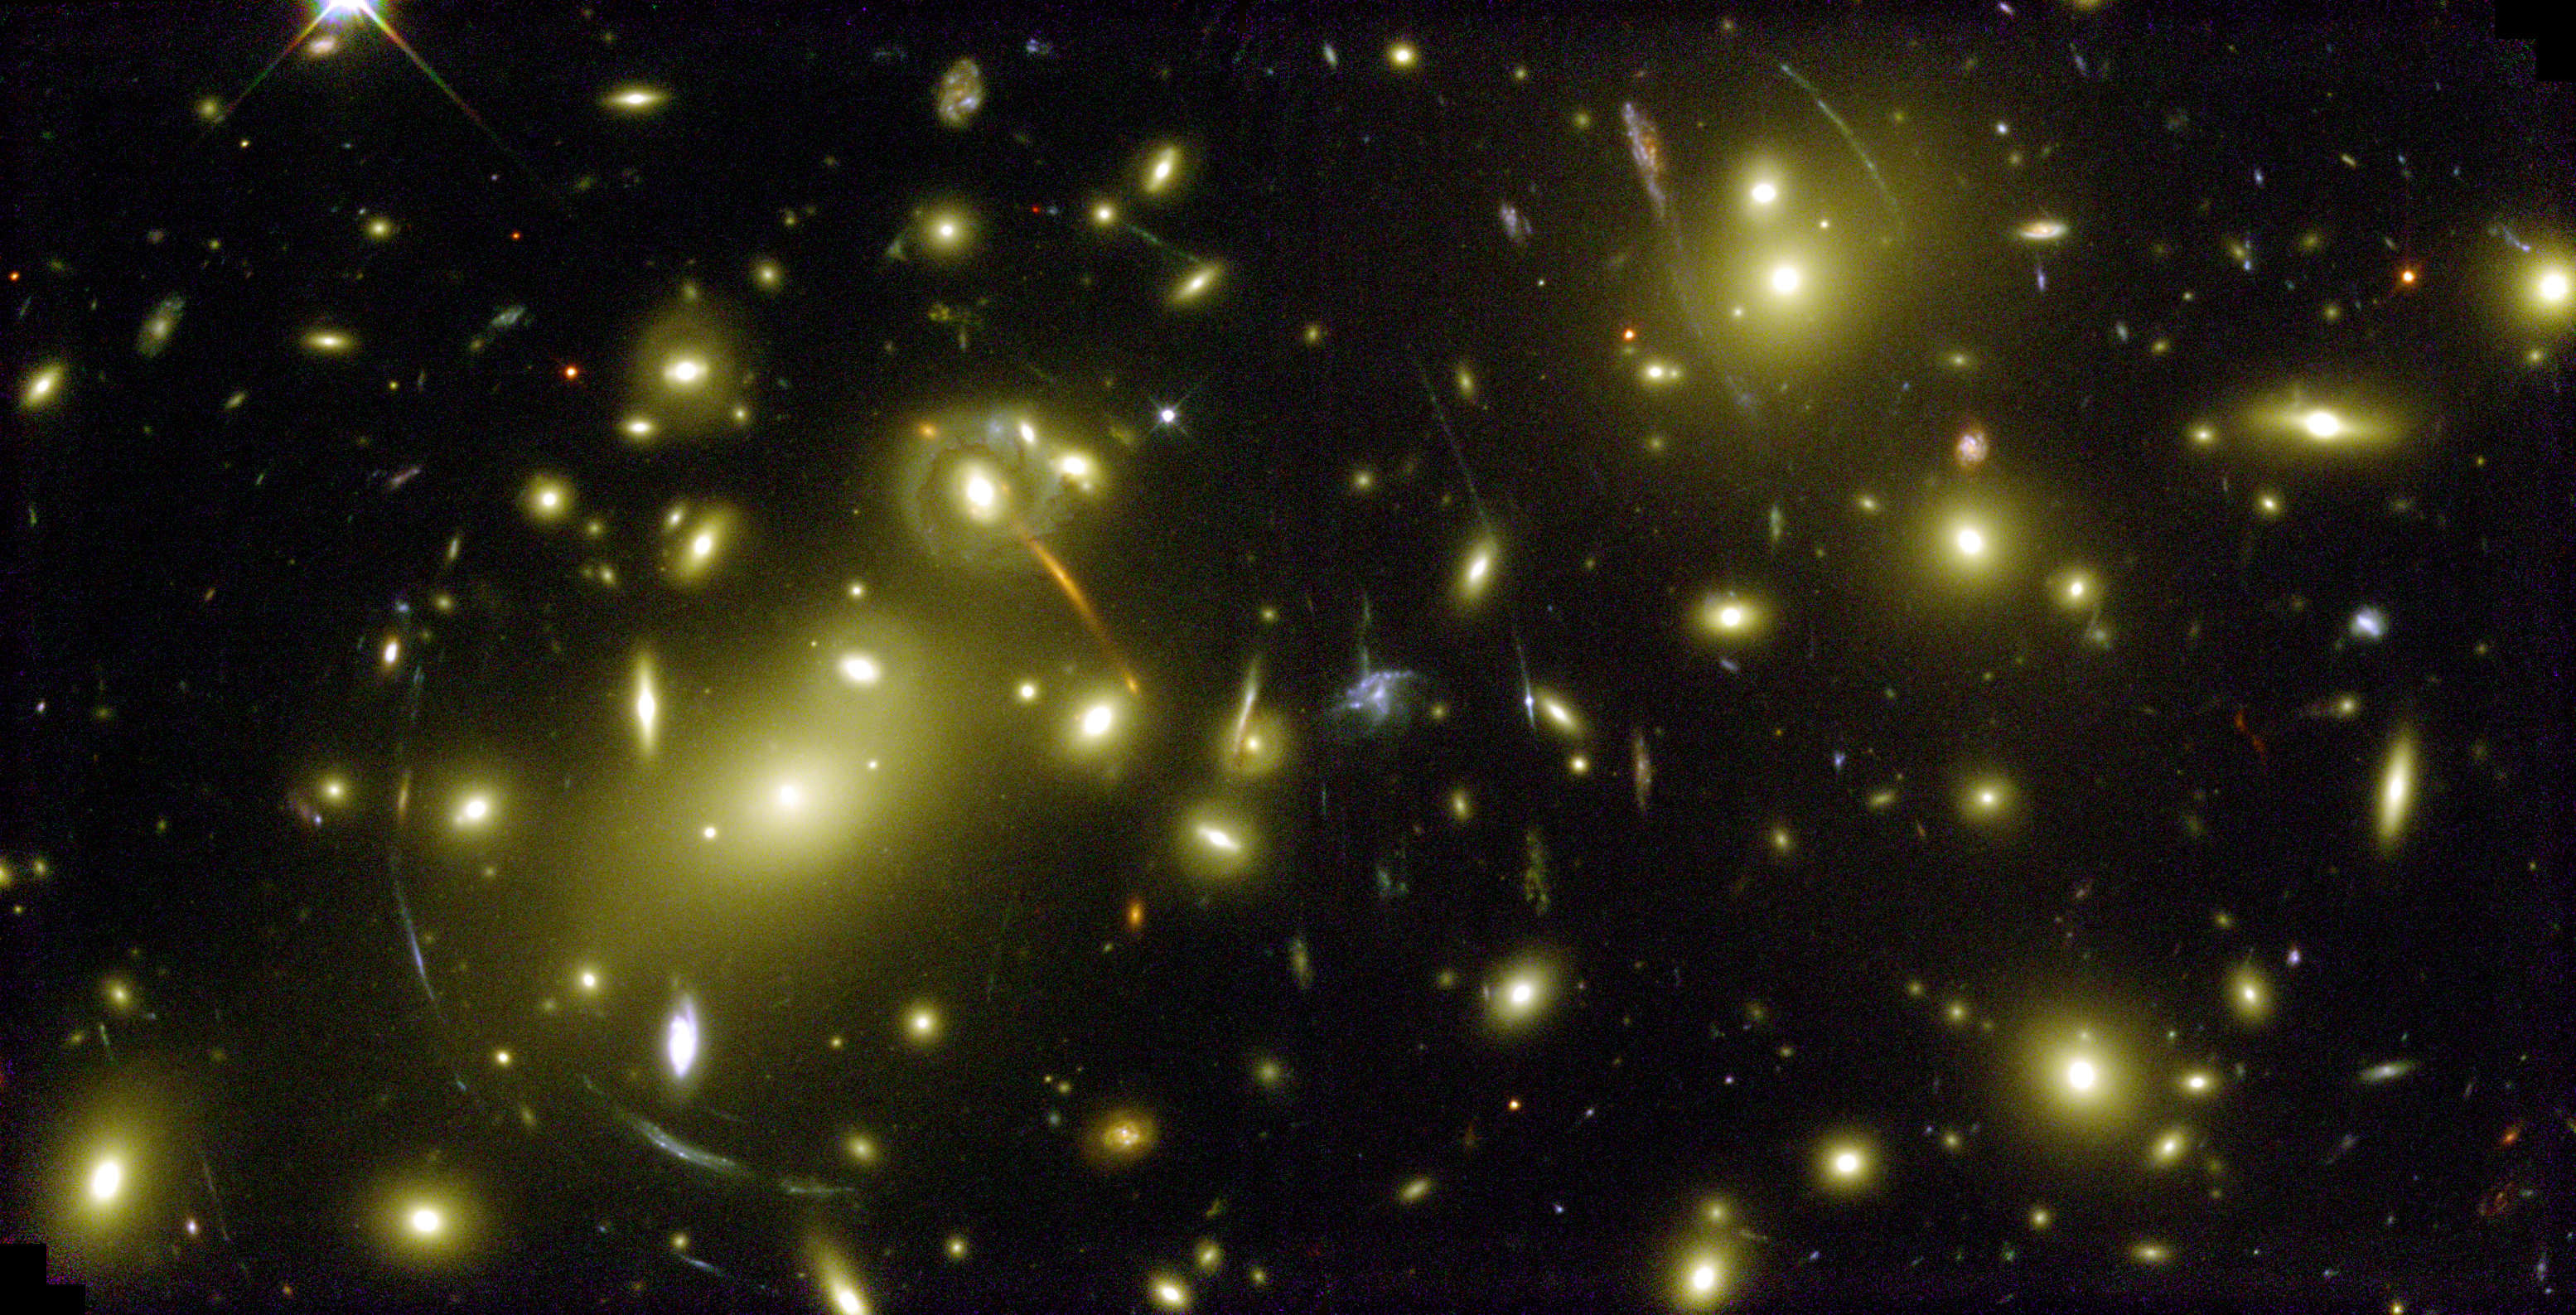
\includegraphics[width=\textwidth]{cluster/images/HSTCI_PR00-08}
  \caption{Galaxiencluster (Abell 2218; NASA, ERO Team)
    \cite{wiki:abell}}
  \label{fig:abell}
\end{figure}

\section{``Normale'' Linse}
\rhead{Normale Linse}
Zuerst einmal ein Rückblick wie eine ``normale'' Linse funktioniert.
Eine ``normale'' Linse nutzt die Brechung zwischen dem Linsenmaterial
und seiner Umgebung aus.  Durch diese Brechung kommt es zu einer
Winkeländerung des Lichtstrahls.  Bei homogenen Materialien mit
bekannten Brechungsindizes kann folgende Formel aus der geometrischen
Optik verwendet werden:

\begin{equation}
  \frac{\sin \varepsilon_1}{\sin \varepsilon_2} = \frac{n_2}{n_1}.
\end{equation}

Darin kommen die Winkel zur Oberflächennormalen im Sinus-Bruch
und die beiden Brechungsindizes vor.  Der
Brechungsindex eines Mediums \(n\), ergibt sich aus der
Lichtgeschwindigkeit im Vakuum \(c\) geteilt durch die
Lichtgeschwindigkeit \(u\) im Medium:

\begin{equation}
  n = \frac{c}{u}.
\end{equation}
\index{Brechungsindex}


\subsection{Prinzip von Huygens}
\rhead{Prinzip von Huygens}
\index{Huygens!Prinzip von}
Wie sich das Licht ausbreitet lässt sich anschaulich mit dem Prinzip
von Huygens aufzeigen.  In der Abbildung \ref{fig:huygens1} ist die
Lichtwellenausbreitung in einem homogenen Medium gezeigt.  Die
Lichtwelle (rote Linie unten) ist nach einem Zeitschritt
(\(\Delta t\)) an der mittleren Position zu finden.  Nach einem
weiteren \(\Delta t\) ist die Lichtwelle an der Position der obersten
roten Linie.  In der Abbildung bewegt sich die Lichtwelle von unten
nach oben.  Weil es sich um ein homogenes Material handelt, sind die
Abstände zwischen den Lichtwellen parallel und immer im gleichen
Abstand.  Das Prinzip von Huygens sagt nun, dass man von jedem Punkt
aus auf einer Lichtwelle (rote Linie), einen Halbkreis in
Ausbreitungsrichtung einzeichnen kann.  Der Halbkreis ist die Distanz,
welche das Licht nach \(\Delta t\) zurückgelegt hat.  Legt man nun
eine Umhüllende um die Halbkreise, erhält man die Position der
Lichtwelle zum neuen Zeitpunkt.

\begin{figure}
  \centering
  %
% Brechung nach dem Prinzip von Huygens


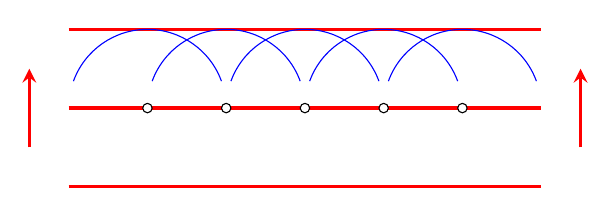
\begin{tikzpicture}

  
  % Delta t
  \foreach \y in {-1,0,1}
    \draw [very thick, color=red] (0,\y) -- (6,\y);

  \foreach \x in {1,2,3,4,5}
    \draw [black, fill=white] (\x,0) circle (.6mm);

  \foreach \x in {1,2,3,4,5}
    \draw [blue] (\x,0) ++ (0,1) arc (90:160:1cm)
                 (\x,0) ++ (0,1) arc (90:20:1cm);

  \draw [very thick, color=red, ->, >=stealth] (-.5,-.5) -- (-.5,0.5);
  \draw [very thick, color=red, ->, >=stealth] (6.5,-.5) -- (6.5,0.5);


\end{tikzpicture}
  \caption{Lichtwellen Ausbreitung nach dem Prinzip von Huygens.}
  \label{fig:huygens1}
\end{figure}

Hat man zwei verschiedenen homogene Materialien, kommt es zur
Brechung, welche auch mit dem Prinzip von Huygens gezeigt werden kann.
In der Abbildung \ref{fig:huygens2} kommt die Lichtwelle von oben
links.  Zum Zeitpunkt in dem die Lichtwelle die beiden Punkte \(A\)
und \(B\) bildet, berührt die Lichtwelle im Punkt \(A\) den
Materialübergang.  Zeichnet man nun die ``Bewegungs-Halbkreise'' ein,
so ist der Halbkreis ausgehend von \(B\) grösser als von \(A\).  Der
Grund dafür ist die höhere Lichtgeschwindigkeit im weissen Medium als
im blauen Medium.  Legt man von \(D\) aus die Tangente an den von
\(A\) ausgehenden Halbkreis, erhält man die Lichtwelle nach
\(\Delta t\).  Es ist gut sichtbar, dass die Lichtwelle
\(\overline{CD}\) gebrochen wurde und nicht parallel zu
\(\overline{AB}\) liegt.

\begin{figure}
  \centering
  \input{cluster/tikz/huygens2.tikz}
  \caption{Brechung nach dem Prinzip von Huygens.}
  \label{fig:huygens2}
\end{figure}

Im Fall der Gravitationslinse gibt es im Weltall natürlich keine starr
begrenzte homogene Bereiche.  Besser zum Vergleich geeignet ist die
Abbildung \ref{fig:huygens3} mit einem inhomogenen Material.  Durch
die tiefere Lichtgeschwindigkeit im blauen Material ist der Abstand
zwischen den Lichtwellen kleiner als im weissen Material, somit biegt
sich der Lichtstrahl.

Da die Lichtgeschwindigkeit in einem Gebiet mit hoher Gravitation
langsamer vergeht, biegen sich Lichtstrahlen in Richtung massen
schwere Objekte.  (Zum Beispiel könnte im Zentrum der blauen Fläche
ein Stern stehen.  Licht, welches nahe dem Stern vorbeigeht, wird in
Richtung des Sterns abgelenkt.)

\begin{figure}
  \centering
  %
% Brechung nach dem Prinzip von Huygens


\begin{tikzpicture}
  [every label/.style={color=black}]

  
  %

  \shade [inner color=blue!50!white, outer color=white] (-.6,0.55) circle (1.5cm);

  \coordinate (A) at (0,0);
  \coordinate (B) at (3,0);
  \draw [very thick, color=red] (A) -- (B);

  \path (B) ++ (97:1cm) coordinate (Bs);
  \path (Bs) ++ ($ (A)!1!187:(B) $) coordinate (As);
  \draw [very thick, color=red] (As) -- (Bs);

  \path (Bs) ++ (104:1cm) coordinate (Bss);
  \path (Bss) ++ ($ (A)!1!194:(B) $) coordinate (Ass);
  \draw [very thick, color=red] (Ass) -- (Bss);

  \draw [very thick, color=red] (A) ++ (0,-1) --++ ($ (B)-(A) $);
  \draw [very thick, color=red] (Bss) ++ (104:1cm) --++ ($ (A)!1!194:(B) $);

  
  % \fill [fill=blue!15!white] (0,0) rectangle (6,-2);
  % \draw [thick] (0,0) -- (6,0);
  % \coordinate[label=below left:$A$] (A) at (3,0);
  % \path (A) ++ (2,0) coordinate[label=below right:$D$] (D);

  % \draw [very thick, color=red, -<, >=stealth] (A) --++ (150:2.5) node(ray1Start){};
  % \path [name path=rayStart] (ray1Start.center) --++ (60:2.5);
  % \path [name path=ray2] (A) ++ (2,0) --++ (150:6);
  % \draw [very thick, color=red, name intersections={of=rayStart and ray2,
  %   by=ray2Start}, -<, >=stealth] (A) ++ (2,0) -- (ray2Start);

  % \path (ray2Start) ++ (-30:2.5) coordinate[label=above:$B$] (B);
  % \draw [color=red] (A) -- (B);


  % \draw [thick, color=blue] (A) ++ (.8,0) arc (0:-180:.8cm);
  % \draw [thick, color=blue]
  %   let \p1 = ($(B)-(D)$)
  %   in (B) ++ (-30:{veclen(\x1,\y1)}) arc (-30:140:{veclen(\x1,\y1)})
  %      (B) ++ (150:{veclen(\x1,\y1)}) coordinate (Bs)
  %      (A) ++ (150:{veclen(\x1,\y1)}) coordinate (As);

  % \draw [color=red] (As) -- (Bs);

  % \node [circle] (circleSmall) at (A) [minimum size=2*.8cm,
  %   inner sep=0]{};
  % \draw [color=red] (D) -- (tangent cs:node=circleSmall, point={(D)},
  %   solution=2) coordinate[label=below left:$C$] (C);


  % \path (C) ++ ($ (C)-(A) $) coordinate (Cs);
  % \path (D) ++ ($ (C)-(A) $) coordinate (Ds);
  % \draw [very thick, color=red, ->, >=stealth] (A) -- (C) -- ($ (C)!1.4!(Cs) $);
  % \draw [very thick, color=red, ->, >=stealth] (D) -- ($ (D)!1.4!(Ds) $);
  % \draw [color=red] (Cs) -- (Ds);

  % \foreach \point in {A,B,C,D}
  %   \draw [black, fill=white] (\point) circle (.6mm);


\end{tikzpicture}
  \caption{Brechung nach dem Prinzip von Huygens in einem inhomogen
    Material.}
  \label{fig:huygens3}
\end{figure}


\section{Gravitationslinse}
\rhead{Gravitationslinse}
\subsection{Einfluss der Gravitation auf die Zeit}
\rhead{Einfluss der Gravitation auf die Zeit}
Als Start wird die Formel \eqref{skript:kruemmung:raumzeitabstand}
\begin{equation*}
  s^2 = -c^2 (t_1-t_2)^2 + (x_1-x_2)^2 + (y_1-y_2)^2 + (z_1-z_2)^2
\end{equation*}
aus dem Abschnitt über den Lichtkegel genommen.

Die Gravitationslinse beugt Lichtwellen, somit ist \(s^2=0\), da sich
die Wirkung mit Lichtgeschwindigkeit ausbreitet.  Wird zur
Vereinfachung \(c=1\) gesetzt, ergibt sich:
\begin{equation*}
  0 = -(t_1-t_2)^2 + (x_1-x_2)^2 + (y_1-y_2)^2 + (z_1-z_2)^2
\end{equation*}
oder anders geschrieben
\begin{equation*}
  0 = -dt^2 + dx^2 + dy^2 + dz^2.
\end{equation*}

Die Lichtwellen bewegen sich in minimalen Wegen, was den Geodäten
entspricht.  Die Lichtablenkung an Sternen und Galaxien befindet sich
im Bereich von schwachen Gravitationsfeldern.  Zu diesen wurden die
\(g_{\mu\nu}\):
\begin{align*}
  g_{00} &= -1 -\frac{2\varphi}{c^2} &g_{kk} &= 1,\quad k=1,2,3
\end{align*}
bereits berechnet (Formel \ref{skript:gravitation:naeherung}).
Das Gravitationspotential \(\varphi\) ist für eine Punktmasse:
\begin{equation*}
  \varphi = -\frac{KM}{r}
\end{equation*}
\(M\) ist die Punktmasse, \(K\) die Gravitationskonstante
(oft als \(G\) bezeichnet) und \(r\) der Abstand zur Punktmasse.
Setzt man dies nun zusammen, erhält man folgende \(g_{\mu\nu}\):
\begin{align*}
  g_{00} &= -1 +\frac{2KM}{rc^2} &g_{kk} &= 1,\quad k=1,2,3.
\end{align*}
Für grosse Abstände \(r\) wird \(g_{00}=-1\).  Was gleich der normalen
Minkowski-Metrik ist.

\begin{beispiel}
  In folgendem soll die Zeitveränderung für Werte unserer Sonne
  berechnet werden.  Die Werte sind:
  \begin{align*}
    K &= \SI{6.67e-11}{\meter\cubed\per\kilogram\per\second\squared}
    &M &= \SI{1.99e30}{\kilogram}
    &c &= \SI{2.99e8}{\meter\per\second}.
  \end{align*}
  Die Zeitveränderung wird nur vom zweiten Teil von \(g_{00}\)
  bestimmt, wobei man erhält:
  \begin{align*}
    \tilde{t} &= \frac{2KM}{rc^2}
    &\left[\tilde{t}\right] &=
                              \si{\meter\cubed\per\kilogram\per\second\squared}
                              \cdot \si{\kilogram}
                              \cdot \si{\per\meter}
                              \cdot \si{\per\meter\squared\second\squared}
                              = 1.
  \end{align*}
  Einen Graphen mit den Werten von \(1\) bis \(0.05\) für
  \(\tilde{t}\) mit dem Abstand \(r\) kann in der Abbildung
  \ref{fig:bsp1} gefunden werden.  Ein \(\tilde{t}\) von \(0.25\)
  entspricht einer Verlangsamung von Wasser.  Je näher bei
  \(\tilde{t}=1\) desto langsamer bewegt sich das Licht, da
  \(g_{00} \rightarrow 0\) wird.  Es ist zu beachten, dass das
  geplotete maximale \(r\) von \SI{60000}{\meter} immer noch innerhalb
  der Sonne ist, da der Sonnenradius \SI{\approx 700e6}{\meter}
  entspricht.
  \begin{figure}
    \centering
    

\begin{tikzpicture}[scale = 1.7]
    \datavisualization[scientific axes = clean,
                     y axis = {grid,
                               label=\(\tilde{t}\) von \(1\) bis \(0.05\),
                               min value = 0,
                               max value = 1},
                     x axis = {grid,
                               label=\(r\) in \si{\meter},
                               min value = 0,
                               max value = 60000},
                     visualize as smooth line/.list={ch1},
                     style sheet=vary hue,
                     %style sheet=vary dashing,
                     %ch1={label in legend={text=Mittenkavität}},
                     ]
                    
  data [set=ch1,headline={x, y}, read from file=cluster/source/bsp1.csv];
\end{tikzpicture}
    \caption{\(\tilde{t}\) von \(1\) bis \(0.05\)}
    \label{fig:bsp1}
  \end{figure}
\end{beispiel}

Im obigen Beispiel ist gut ersichtlich, wie schnell der Einfluss der
Gravitation abnimmt.  Eine Linse mit dieser Eigenschaft müsse so
geformt sein, wie ein Weinglasboden.  In der Abbildung
\ref{fig:ModelGravLinse} sind drei Beispielkonstellationen zu sehen.
Ist der Weinglasboden in einer Linie mit der Kerze (unten links)
erhält man ein Einsteinring ähnliches Gebilde.  Bei einem gekippten
Boden (oben rechts) erhält man beinahe ein Einsteinkreuz.  Und unten
rechts sieht man ein Beispiel was passiert, wenn die Linse und die
Quelle nicht in einer Linie stehen (wie im Cluster Bild
\ref{fig:abell}).

\begin{figure}
  \centering
  \includegraphics[width=\textwidth]{cluster/images/model_grav_lens}
  \caption{Model einer Gravitationslinse (Boden eines Weinglases)
    \cite{standford:ModelGravLens}}
  \label{fig:ModelGravLinse}
\end{figure}

\subsection{Euler-Lagrange}
\rhead{Euler-Lagrange}
\index{Euler-Lagrange-Gleichungen}
Um die Lichtablenkung zu berechnen, benötigt man den Weg des Lichts
und nicht nur wie stark die Lichtgeschwindigkeit abgebremst wird.  Das
Licht nimmt den Weg mit der kürzesten Laufzeit.  Aus der Physik kennt
man, dass die Zeit gleich der Strecke durch die Geschwindigkeit ist:
\begin{equation*}
  t = \frac{s}{v}.
\end{equation*}

Für den Weg des Lichts muss man somit jedes Wegstück mit seiner
Geschwindigkeit dividieren und all diese Stückchen zusammen addieren.
Das Licht nimmt nun den Weg, in welchem es die kürzeste Laufzeit hat.
Um eine Strecke zu minimieren, kann man Euler-Lagrange verwenden,
welche ein Integral der Form
\begin{equation*}
  I = \int\limits_{t_0}^{t_1}\! F\bigl(x^{\alpha}(t), \dot{x}^{\alpha}(t),t\bigr)d t
\end{equation*}
benötigt.  Das Integral soll die Zeit minimieren, somit muss es einen
Weg geteilt durch eine Geschwindigkeit im Integral geben.  Eine
Möglichkeit ist folgendes Integral:
\begin{equation}
  I = \int\! \sqrt{\dot{x}(l)^2+\dot{y}(l)^2+\dot{z}(l)^2} \cdot
  \frac{n\bigl(x(l),y(l),z(l)\bigr)}{c} d l.
\end{equation}

Der Wert unter der Wurzel entspricht dem Wegstück während eines
Integrationsschritts.  Die Division entspricht eins durch die
Geschwindigkeit.  Somit erhält man im Integral eine Zeit, welche über
den gesamten Weg integriert der Wegzeit des Lichts entspricht.  Da die
Lichtgeschwindigkeit \(c\) unabhängig von der Position ist, kann man
den Bruch vor das Integral nehmen:
\begin{equation}
  I = \frac{1}{c}\int\! \sqrt{\dot{x}(l)^2+\dot{y}(l)^2+\dot{z}(l)^2}
  \cdot n\bigl(x(l),y(l),z(l)\bigr) d l.
\end{equation}
Des Weiteren benötigt man für Euler-Lagrange nur den Teil im Integral:
\begin{equation}
  L = \sqrt{\dot{x}(l)^2+\dot{y}(l)^2+\dot{z}(l)^2}
  \cdot n\bigl(x(l),y(l),z(l)\bigr).
\end{equation}
Da die Wurzel die folgenden Rechenschritte verkompliziert, wird sie
quadriert, was das Extremum nicht verändert.  Dieser Schritt wurde
bereits im Abschnitt
\ref{skript:geodaeten:subsection:Parametrisierung} angewendet.  Weiter
wird die Abhängigkeit von \(l\) nicht mehr geschrieben, was es
natürlich bleibt:
\begin{equation}
  F = L^2 = (\dot{x}^2+\dot{y}^2+\dot{z}^2)n^2.
\end{equation}

Für Euler-Lagrange muss man nun dieses \(F\) ableiten, im folgenden
nur mit \(x\) gezeigt:
\begin{equation}
  \label{eq:cluster:euler}
  0 = \frac{\partial F}{\partial x} - \frac{d}{d l} \frac{\partial
    F}{\partial \dot{x}}.
\end{equation}
Die Ableitungen sind
\begin{align*}
  \frac{\partial F}{\partial x} &= (\dot{x}^2+\dot{y}^2+\dot{z}^2) 2n
                                  \frac{\partial n}{\partial x}\\
  \frac{\partial F}{\partial\dot{x}} &= 2\dot{x}n^2\\
  \frac{d}{d l}\frac{\partial F}{\partial\dot{x}} &= 2\ddot{x}n^2 + 4\dot{x}n
                                \left(\frac{\partial n}{\partial x}\dot{x} +
                                \frac{\partial n}{\partial y}\dot{y} +
                                \frac{\partial n}{\partial z}\dot{z} \right).
\end{align*}
Setzt man die obigen Berechnungen in \ref{eq:cluster:euler} ein und
löst diese Formel nach \(\ddot{x}\) auf, erhält man:
\begin{equation}
  \ddot{x} = (-\dot{x}^2+\dot{y}^2+\dot{z}^2)
  \frac{1}{n}\frac{\partial n}{\partial x} -
  2\dot{x}\dot{y} \frac{1}{n}\frac{\partial n}{\partial y} -
  2\dot{x}\dot{z} \frac{1}{n}\frac{\partial n}{\partial z}.
\end{equation}
Mit der Hilfe der logarithmischen Differentiation
\begin{equation*}
  \frac{1}{n} \frac{\partial n}{\partial x} = \frac{\partial \ln
    n}{\partial x}
\end{equation*}
kann man die Formel weiter vereinfachen:
\begin{equation}
  \ddot{x} = (-\dot{x}^2+\dot{y}^2+\dot{z}^2) \frac{\partial \ln
    n}{\partial x} - 2\dot{x}\dot{y} \frac{\partial \ln n}{\partial y}
  - 2\dot{x}\dot{z} \frac{\partial \ln n}{\partial z}.
\end{equation}
Normalerweise ist ein Logarithmus nicht der einfachste Ansatz.  Die
Vereinfachung entsteht durch die spezielle Form von \(n\)
\begin{equation*}
  n \approx 1-\frac{2\varphi}{c^2}
\end{equation*}
und weil
\begin{equation*}
  \frac{\varphi}{c^2} \ll 1
\end{equation*}
ergibt sich
\begin{equation*}
  \ln n \approx -\frac{2\varphi}{c^2}.
\end{equation*}

Somit muss man nun keine partielle Ableitung von \(\ln n\), sondern von
\(-\frac{2\varphi}{c^2}\) durchführen (d.h. man braucht
\(\nabla\varphi=\) Gravitationskraft).  In einem Beispiel soll dies in
2D gezeigt werden.

\begin{beispiel}
  Im Folgenden wird die Lichtablenkung in einem zwei dimensionalen
  Raum numerisch berechnet.  Als \(\varphi\) wird eine Punktquelle
  verwendet:
  \begin{equation*}
    \varphi = -\frac{KM}{r}.
  \end{equation*}
  Wobei
  \begin{equation*}
    r = \sqrt{(x-x_L)^2+(y-y_L)^2}
  \end{equation*}
  der Abstand zwischen dem aktuellen Punkt und der Linse ist.

  Berechnet man mit Hilfe von Maxima Euler-Lagrange nach den beiden
  Koordinatenachsen, erhält man:
  \begin{align*}
    \ddot{x} &= -\frac{2(-\dot{x}^2+\dot{y}^2)(x-x_L)KM}
               {c^2\sqrt{(x-x_L)^2+y^2}\,^3}+
               \frac{4\dot{x}y\dot{y}KM}{c^2\sqrt{(x-x_L)^2+y^2}\,^3}\\
    \ddot{y} &= +\frac{4\dot{x}\dot{y}(x-x_L)KM}{c^2\sqrt{(x-x_L)^2+y^2}\,^3}
               - \frac{2(\dot{x}^2-\dot{y}^2)yKM}
               {c^2\sqrt{(x-x_L)^2+y^2}\,^3}.
  \end{align*}
  In diesem Beispiel befindet sich die Gravitationslinse auf \(x=0\),
  somit vereinfacht sich \(y-y_L\) zu \(y\).  Die soeben erhaltenen
  Formeln kann man in dieser Form noch nicht verwenden.  Man hat ein
  Differentialgleichungssystem zweiter Ordnung.  Was von geläufigen
  Computer Algorithmen nicht gelöst werden kann, da sie ein DGL-System
  erster Ordnung benötigen.

  Mit Substitution kann man eine Differentialgleichung zweiter Ordnung
  in ein DGL-System erster Ordnung überführen.  Macht man diese
  Substitution mit beiden Formeln, erhält man ein Gleichungssystem
  erster Ordnung, welche beide Formeln enthält.  Wählt man folgende
  Substitutionen
  \begin{align*}
    x_1 &= x &x_2 &= \dot{x} &x_3 &= y &x_4 &= \dot{y}
  \end{align*}
  kann man die beiden Formeln in eine brauchbare Form bringen.  Die
  gängigen Algorithmen fordern die Ableitungen von \(x_k\) als
  Parametern:
  \begin{align*}
    \dot{x}_1 &= x_2\\
    \dot{x}_2 &= -\frac{2\left(-x_2^2+x_4^2\right)\bigl(x_1-x_L\bigr)KM}
                {c^2\sqrt{\bigl(x_1-x_L\bigr)^2+x_3^2}\,^3}
                + \frac{4 x_2x_3x_4 KM}
                {c^2\sqrt{\bigl(x_1-x_L\bigr)^2+x_3^2}\,^3}\\
    \dot{x}_3 &= x_4\\
    \dot{x}_4 &= +\frac{4x_2x_4\bigl(x_1-x_L\bigr)KM}
                {c^2\sqrt{\bigl(x_1-x_L\bigr)^2+x_3^2}\,^3}
                - \frac{2 \left(x_2^2-x_4^2\right) x_3 KM}
                {c^2\sqrt{\bigl(x_1-x_L\bigr)^2+x_3^2}\,^3}.
  \end{align*}

  In Octave wird \(x_k\) zu \texttt{x(k)}, was zu folgendem Code
  führt:
  \lstinputlisting[style=Octave]{cluster/source/dglSubCode.m}

  Setzt Man nun die Werte
  \begin{align*}
    x_L &\approx \SI{150e6}{\kilo\meter} &M &\approx
                                              \SI{2e30}{\kilogram}
    &R &\approx \SI{700e3}{\kilo\meter}
  \end{align*}
  der Sonne ein,
  erhält man eine Winkeländerung von \(\approx \SI{1.75}{''}\),
  vergleicht man dies mit dem Wert aus der Literatur von
  \(\SI{1.75}{''}\) (\cite{misner1973gravitation} S.446), scheint
  dieses Vorgehen ziemlich adäquat.

  Im Graphen \ref{fig:lichtablenkungSonne} ist der numerisch
  berechnete Lichtweg dargestellt.  Der Beobachter ist im Punkt (0,0)
  und die Sonne im Punkt (\SI{1.5e11}{\meter},0).  Der Lichtpfad
  startet von der Erde aus so, dass man direkt am Sonnenradius
  vorbeischaut.  Da die Ablenkung nur \SI{1.75}{''} ist, sieht der Lichtweg
  von Auge betrachtet wie eine gerade Strecke aus.  (Eine Bogensekunde
  ist ein 3600stel eines Grades.)

  Nimmt man zur Berechnung eine schwerere Sonne an, ist die
  Lichtablenkung auch von Auge gut zu sehen.  In der Abbildung
  \ref{fig:lichtablenkung300Sonne} ist die Sonne 300 mal schwerer (bei
  gleichem Radius) und in \ref{fig:lichtablenkung600Sonne} sogar 600
  mal mehr.

  \begin{figure}
    \centering
    \begin{tikzpicture}[scale = 1.7]
      \datavisualization[scientific axes = clean,
                         y axis = {grid,
                                   label=\(y\) in \si{\meter},
                                   min value = 0,
                                   max value = 1.5e9},
                         x axis = {grid,
                                   label=\(x\) in \si{\meter},
                                   min value = 0,
                                   max value = 3e11},
                         visualize as smooth line/.list={ch1},
                         % ch1={style=very thick},
                         style sheet=vary hue,
                         % style sheet=vary dashing,
                         % ch1={label in legend={text=Mittenkavität}},
                        ]
                    
      data [set=ch1,headline={x, y}, read from file=cluster/source/lichtablenkungSonne.csv];
    \end{tikzpicture}
    \caption{Lichtablenkung an der Sonne}
    \label{fig:lichtablenkungSonne}
  \end{figure}
  
  \begin{figure}
    \centering
    \begin{tikzpicture}[scale = 1.7]
      \datavisualization[scientific axes = clean,
                         y axis = {grid,
                                   label=\(y\) in \si{\meter},
                                   min value = 0,
                                   max value = 1.5e9},
                         x axis = {grid,
                                   label=\(x\) in \si{\meter},
                                   min value = 0,
                                   max value = 3e11},
                         visualize as smooth line/.list={ch1},
                         % ch1={style=very thick},
                         style sheet=vary hue,
                         % style sheet=vary dashing,
                         % ch1={label in legend={text=Mittenkavität}},
                        ]
                    
      data [set=ch1,headline={x, y}, read from file=cluster/source/lichtablenkung300Sonne.csv];
    \end{tikzpicture}
    \caption{Lichtablenkung an 300 Sonnenmassen}
    \label{fig:lichtablenkung300Sonne}
  \end{figure}
  
  \begin{figure}
    \centering
    \begin{tikzpicture}[scale = 1.7]
      \datavisualization[scientific axes = clean,
                         y axis = {grid,
                                   label=\(y\) in \si{\meter},
                                   min value = 0,
                                   max value = 1.5e9},
                         x axis = {grid,
                                   label=\(x\) in \si{\meter},
                                   min value = 0,
                                   max value = 3e11},
                         visualize as smooth line/.list={ch1},
                         % ch1={style=very thick},
                         style sheet=vary hue,
                         % style sheet=vary dashing,
                         % ch1={label in legend={text=Mittenkavität}},
                        ]
                    
      data [set=ch1,headline={x, y}, read from file=cluster/source/lichtablenkung600Sonne.csv];
    \end{tikzpicture}
    \caption{Lichtablenkung an 600 Sonnenmassen}
    \label{fig:lichtablenkung600Sonne}
  \end{figure}
\end{beispiel}

Im vorherigen Beispiel sieht man gut, dass die Lichtstrahlen bis
praktisch zur Sonne eine Gerade darstellen, dann abgebogen werden und
wieder in einer Gerade weiterfliegen.  Stellt man nur diese Ablenkung
dar (\ref{fig:lichtablenkung600SonneZoom}) ist das noch besser
sichtbar.

\begin{figure}
  \centering
  \begin{tikzpicture}[scale = 1.7]
    \datavisualization[scientific axes = clean,
                       y axis = {grid,
                                 label=\(y\) in \si{\meter},
                                 min value = 6.5e8,
                                 max value = 7e8},
                       x axis = {grid,
                                 label=\(x\) in \si{\meter},
                                 min value = 1.4e11,
                                 max value = 1.6e11},
                       visualize as smooth line/.list={ch1},
                       % ch1={style=very thick},
                       style sheet=vary hue,
                       % style sheet=vary dashing,
                       % ch1={label in legend={text=Mittenkavität}},
                      ]
                    
    data [set=ch1,headline={x, y}, read from file=cluster/source/zoomLichtablenkung600Sonne.csv];
  \end{tikzpicture}
  \caption{Lichtablenkung an 600 Sonnenmassen (Zoom)}
  \label{fig:lichtablenkung600SonneZoom}
\end{figure}

Das Verhalten, dass über eine lange Strecke nichts passiert, erschwert
die nummerische Berechnung.  Die Algorithmen ode23 und ode45 in Octave
waren nicht in der Lage den Weg zu berechnen.  Hingegen konnte die
Lichtablenkung im Beispiel oben mit ode23s aus Octave berechnet
werden.  Dieser Algorithmus ist fähig steife Probleme zu berechnen.
Solche Probleme nennt man steif, wenn eine tiefe Frequenz von einer
hohen Frequenz überlagert wird.  Im weiteren Sinn ist dieses Problem
steif, da zwischen Beobachter, Gravitationslinse und Quelle sehr
grosse Abstände vorhanden sind, in denen nichts passiert.  Zum Lösen
berechnet ode23s auf der gesamten vorgegebenen Strecke Punkte.  Für
Sonnenabstände ist dies noch gut berechenbar, für Galaxienabstände
jedoch nicht.

\subsection{Bildverzerrung}
\rhead{Bildverzerrung}
Möchte man nun ein Bild der Lichtablenkung erzeugen, muss man für
jedes Pixel den Lichtweg simuliert.  Wenn man den einfachsten Fall der
Punktquelle beibehält, kann man die Symmetrie ausnützen und muss somit
nur ein Achtel der Pixelauflösung berechnen.

Für die Simulation wurde wieder der Abstand von der Erde zur Sonne
verwendet.  Um die Lichtablenkung noch zu verstärken, wurde die
tausendfache Sonnenmasse bei gleichem Radius angenommen.  Der
Pixelabstand in der Sonnenebene liegt bei \SI{10e6}{\meter}.  Das
Hintergrundbild, die Andromeda Galaxie aus Abbildung \ref{fig:m31},
ist in rund 6.8 fachem Sonnenabstand von der Erde aus platziert.  Der
Pixelabstand wurde gleich gewählt.

\begin{figure}
  \centering
  \includegraphics[width=\textwidth]{cluster/images/m31_comolli_2193}
  \caption{Andromeda Galaxie M31 \cite{nasa:andromedaM31}}
  \label{fig:m31}
\end{figure}

In der Abbildung \ref{fig:einsteinringSim} sieht man, wie das Zentrum
der Galaxie zu einem Ring verzogen wird.  Das schwarze Zentrum in der
Abbildung ist die Position der ``Sonne''.  Die Abbildung hat eine
Auflösung von \(300\times300\) Pixel und benötigte gut eineinhalb Tage
Berechnungszeit bei vier Kernen mit Hyper-Threading.

\begin{figure}
  \centering
  \includegraphics[width=.6\textwidth]{cluster/images/einsteinring}
  \caption{Bildverzerrung durch 1000 Sonnenmassen}
  \label{fig:einsteinringSim}
\end{figure}

\printbibliography[heading=subbibliography]
\end{refsection}



\printbibliography[heading=subbibliography]
\end{refsection}



